
\refstepcounter{Exercise}
\clearpage\subsection*{\theExercise Weblioのウェブページをスクレイピングする}
\addtocounter{Exercise}{-1}\refstepcounter{Exercise}\label{E:Weblio}
\noindent 考え方

まずは、ウェブブラウザでWeblioのページを見てみよう。
授業で使用したホームページを開いてください。
\textbf{({\textasciitilde}/08/links.html)}

Weblioをクリックします。

\begin{center}
    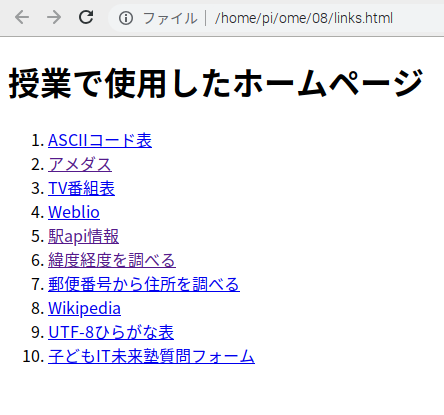
\includegraphics[width=0.5\textwidth]{textbook-img017.png}
\end{center}

Weblioのウェブページが開きます。
このページの検索欄に検索したいワードを入れて検索をすると結果がでてきます。
まずは、適当に検索してみましょう。

\begin{center}
    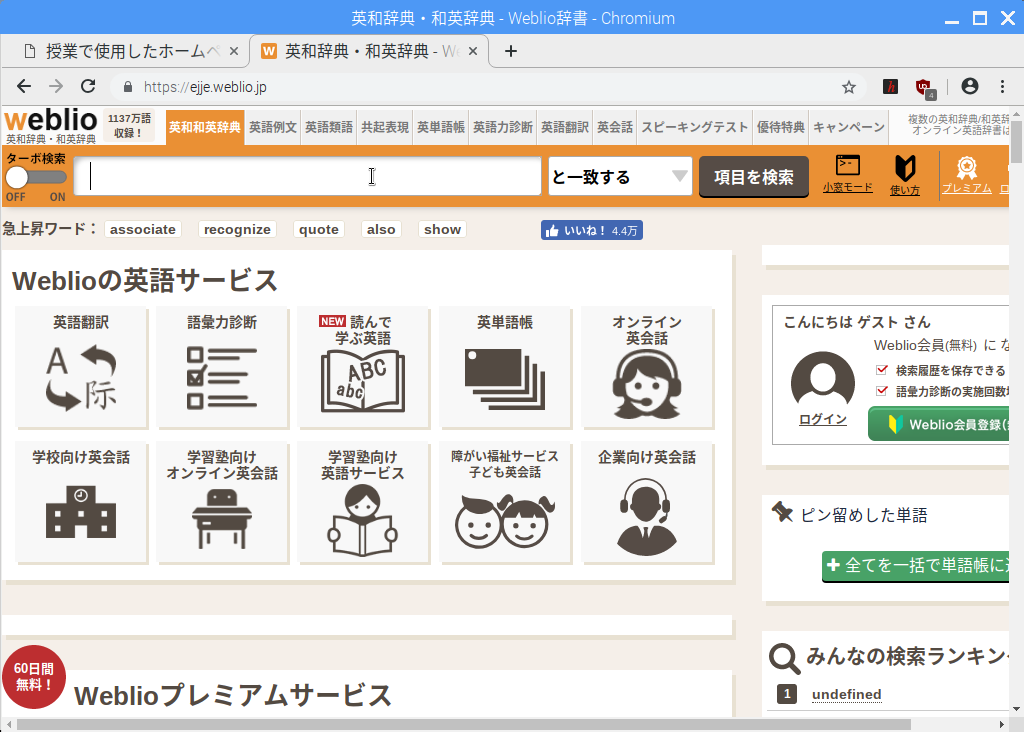
\includegraphics[width=0.8\textwidth]{textbook-img045.png}
\end{center}

\clearpage
試しに”hello”と検索してみました。結果の画面はこのような感じです。
\begin{center}
    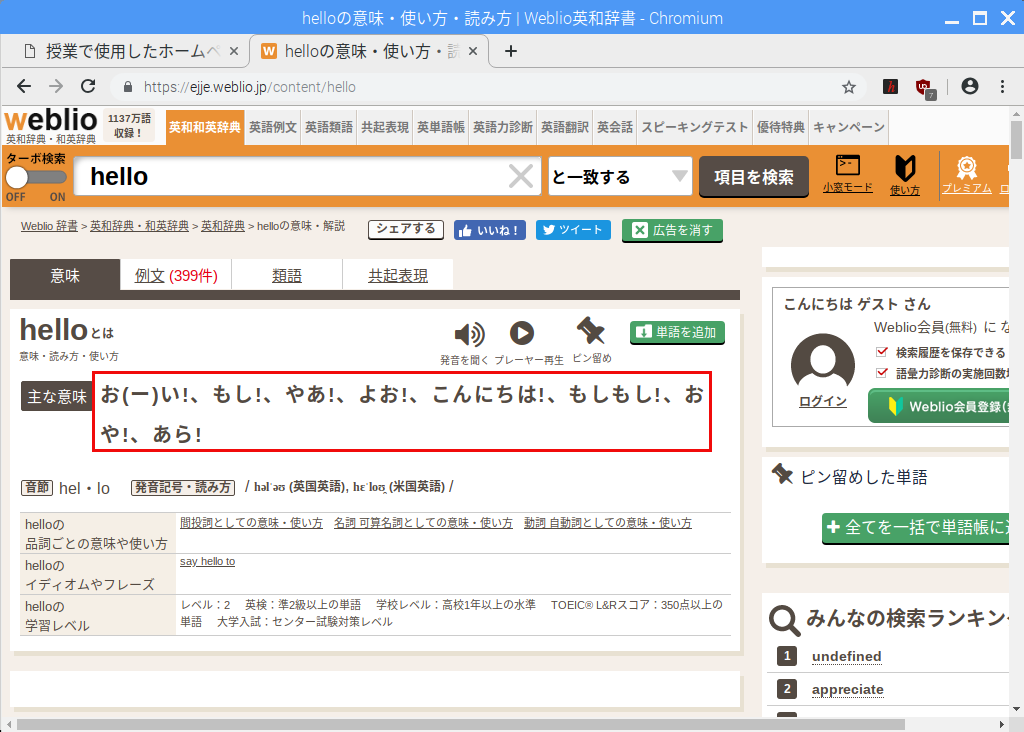
\includegraphics[width=0.8\textwidth]{textbook-img046.png}
\end{center}
今回取得する情報は、検索ワードに対応する主な意味です。

まずはプログラムを動かしてみましょう。

ターミナルを開いて

hsed

と実行してスクリプトエディタを開きます。

\begin{center}
    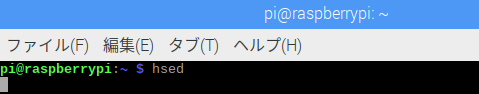
\includegraphics[width=0.9\textwidth]{textbook-img013.png}
\end{center}

\clearpage
HSPスクリプトエディタが開くので

ファイル → 開く..\ をクリックして\textbf{{\textasciitilde}/08/weblio.hsp}を開きます。

プログラムが表示されます。

\begin{center}
    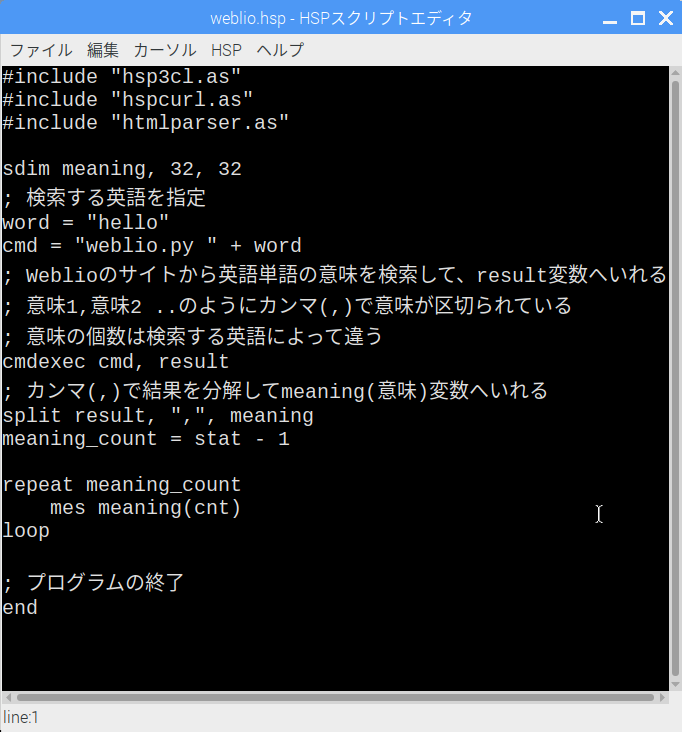
\includegraphics[width=0.7\textwidth]{textbook-img047.png}
\end{center}

F5を押して実行してみましょう。

実行結果はターミナルに表示されます

\begin{center}
    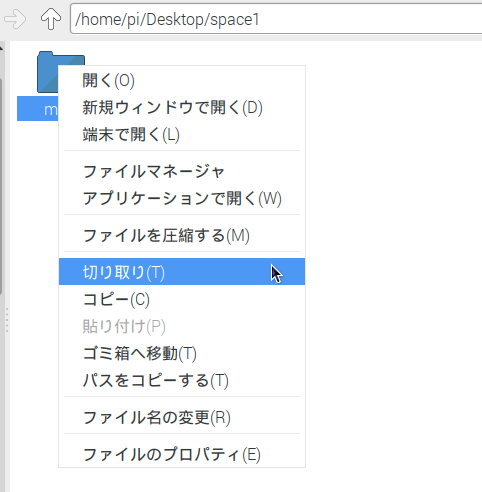
\includegraphics[width=0.7\textwidth]{textbook-img048.png}
\end{center}

\clearpage
ブラウザの表示とプログラムの実行結果を比べてみてください。
”、”で区切られていた意味が表示されています。
\begin{center}
    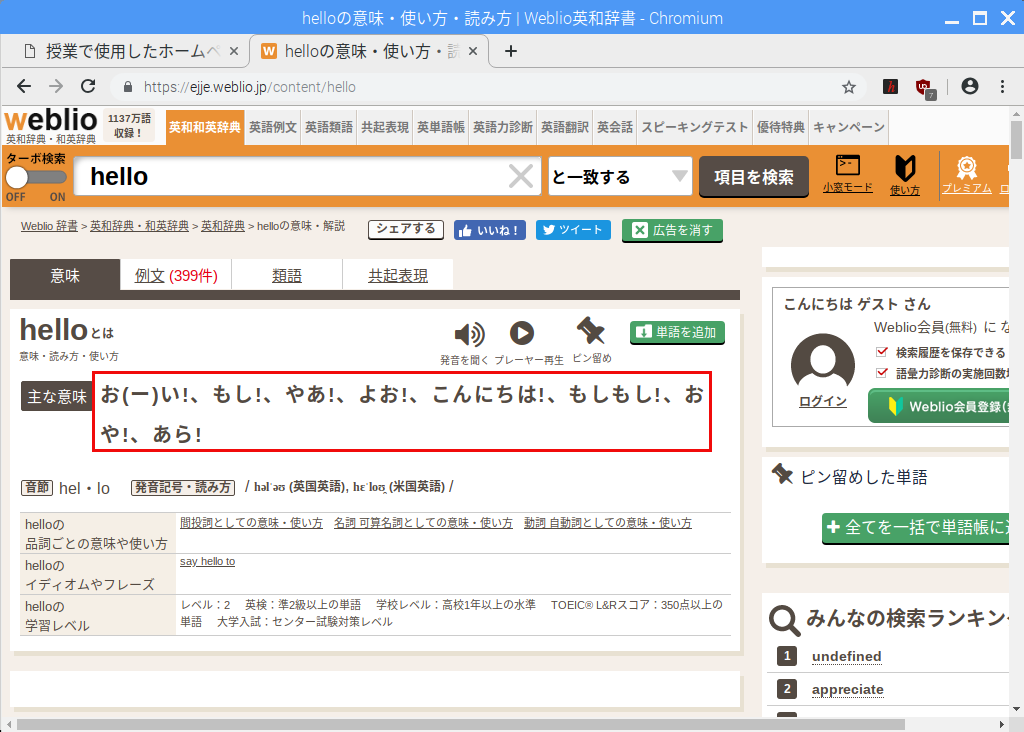
\includegraphics[width=0.9\textwidth]{textbook-img046.png}
\end{center}

\refstepcounter{Question}
\subsection*{\theQuestion\label{Q:weblio}}
7行目のword=”hello”で検索する英語を指定しています。
この変数を自分の検索したい英語にして実行してみましょう。

\ \ HINT : word=”raspberry”

\refstepcounter{Exercise}
\clearpage
\subsection*{\theExercise 位置情報のから近くの駅をスクレイピング}
\addtocounter{Exercise}{-1}\refstepcounter{Exercise}\label{E:station}
\noindent 考え方

まずは、ウェブブラウザで駅検索API情報のページを見てみよう。
授業で使用したホームページを開いてください。
\textbf{({\textasciitilde}/08/links.html)}

駅api情報をクリックします。

\begin{center}
    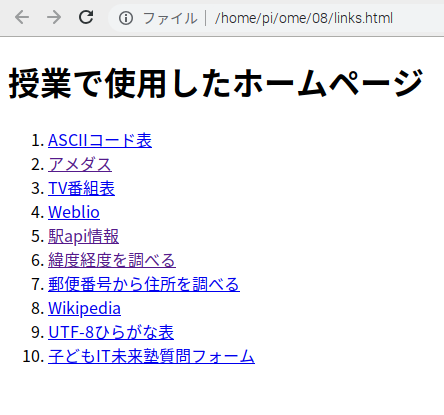
\includegraphics[width=0.5\textwidth]{textbook-img017.png}
\end{center}

駅api情報のウェブページが開きます。
今回使用するのは\ruby{最寄}{もよ}り駅取得 APIです

\begin{center}
    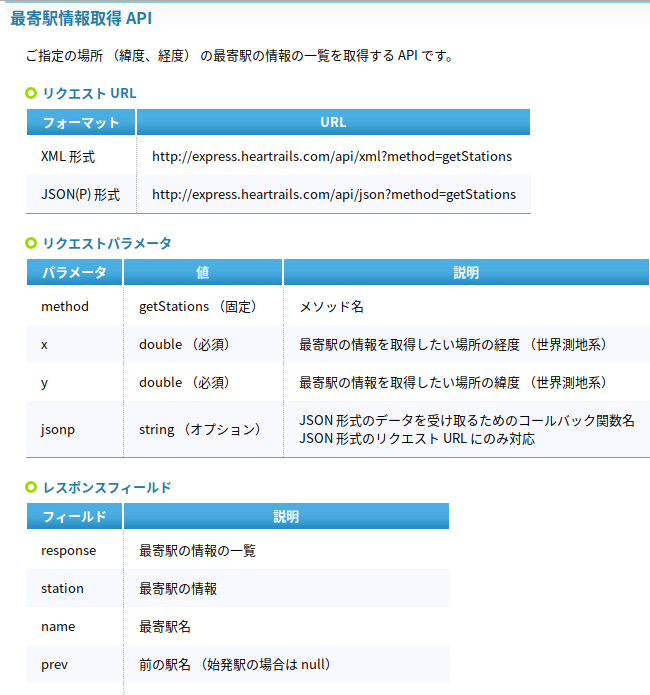
\includegraphics[width=0.6\textwidth]{textbook-img049.png}
\end{center}

\clearpage
まずはプログラムを動かしてみましょう。

ターミナルを開いて

hsed

と実行してスクリプトエディタを開きます。
\begin{center}
  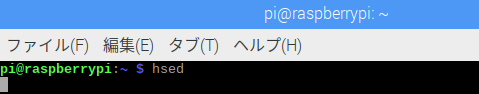
\includegraphics[width=\textwidth]{textbook-img013.png}
\end{center}
HSPスクリプトエディタが開くので

ファイル → 開く..\ をクリックして\textbf{{\textasciitilde}/08/eki.hsp}を開きます。

プログラムが表示されます。

\begin{center}
    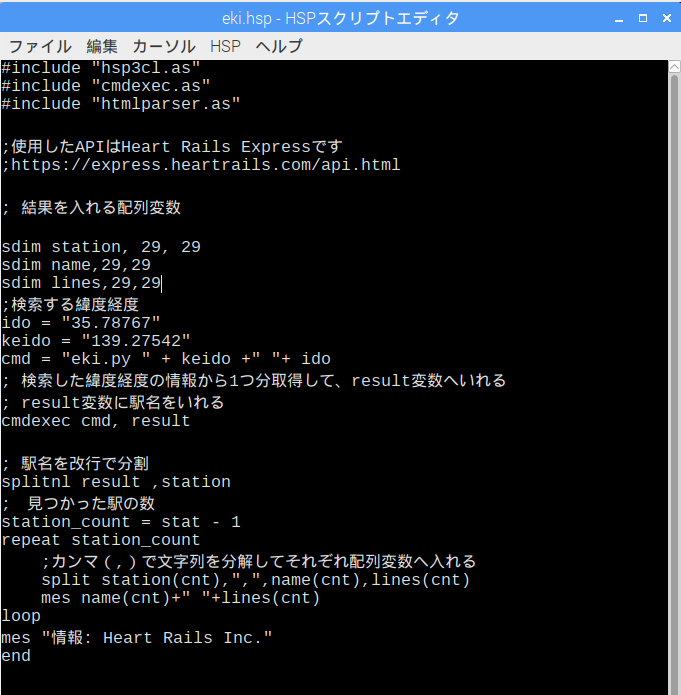
\includegraphics[width=13.377cm]{textbook-img050.png}
\end{center}

\clearpage
F5を押して実行してみましょう。実行結果はターミナルに表示されます
\begin{center}
    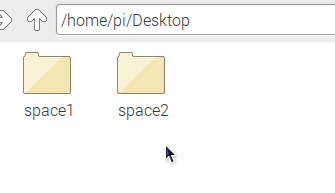
\includegraphics[width=0.8\textwidth]{textbook-img051.png}
\end{center}
ブラウザの表示\\(
\textbf{http://express.heartrails.com/api/xml?method=getStations\&x=139.27542\&y=35.78767}
)とプログラムの実行結果を比べてみてください。
指定した位置に近い駅の名前、その駅の路線名が順に表示されています。

\begin{center}
    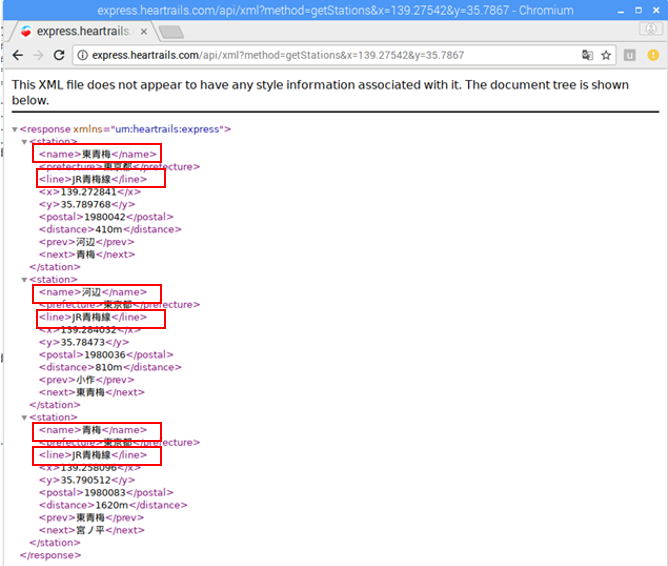
\includegraphics[width=0.8\textwidth]{textbook-img052.png}
\end{center}


\refstepcounter{Question}
\clearpage
\subsection*{\theQuestion\label{Q:station}}
サンプルプログラムでは、青梅市役所の近くの駅名を取得していました。
次は、自分の好きなもしくは知っている場所を指定してみましょう。
\ruby{緯度}{いど}\ruby{経度}{けいど}は、授業で使用したウェブページ\textbf{({\textasciitilde}/08/links.html)}を開いて、

緯度経度を調べるをクリックします。
\begin{center}
    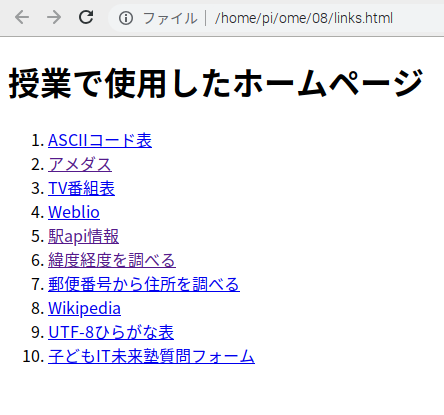
\includegraphics[width=0.5\textwidth]{textbook-img017.png}
\end{center}

フォームで調べたい場所(今回は青梅市役所)を検索(GPS\ruby{座標}{ざひょう}検索)します。
\begin{center}
    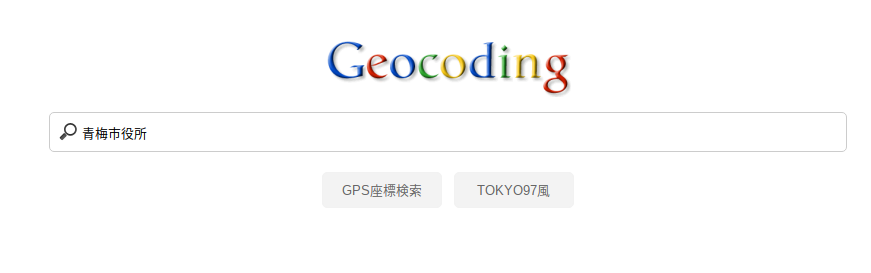
\includegraphics[width=0.8\textwidth]{textbook-img053.png}
\end{center}

\begin{center}
    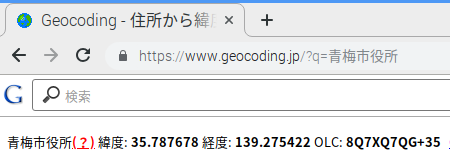
\includegraphics[width=0.5\textwidth]{textbook-img054.png}
\end{center}

検索結果に緯度、経度の数字があります。これをプログラムの
\begin{center}
\begin{boxedminipage}{7.959cm}
Ido=”35.78767”

keido=”139.27542”
\end{boxedminipage}
\end{center}

とすると青梅市役所の最寄りの駅とその路線情報を取得して表示することができます。
